Para activar una luz desde una placa Arduino, usaremos un relé que active una
luz alimentada externamente. El montaje quedaría como se muestra en la
fotografía:

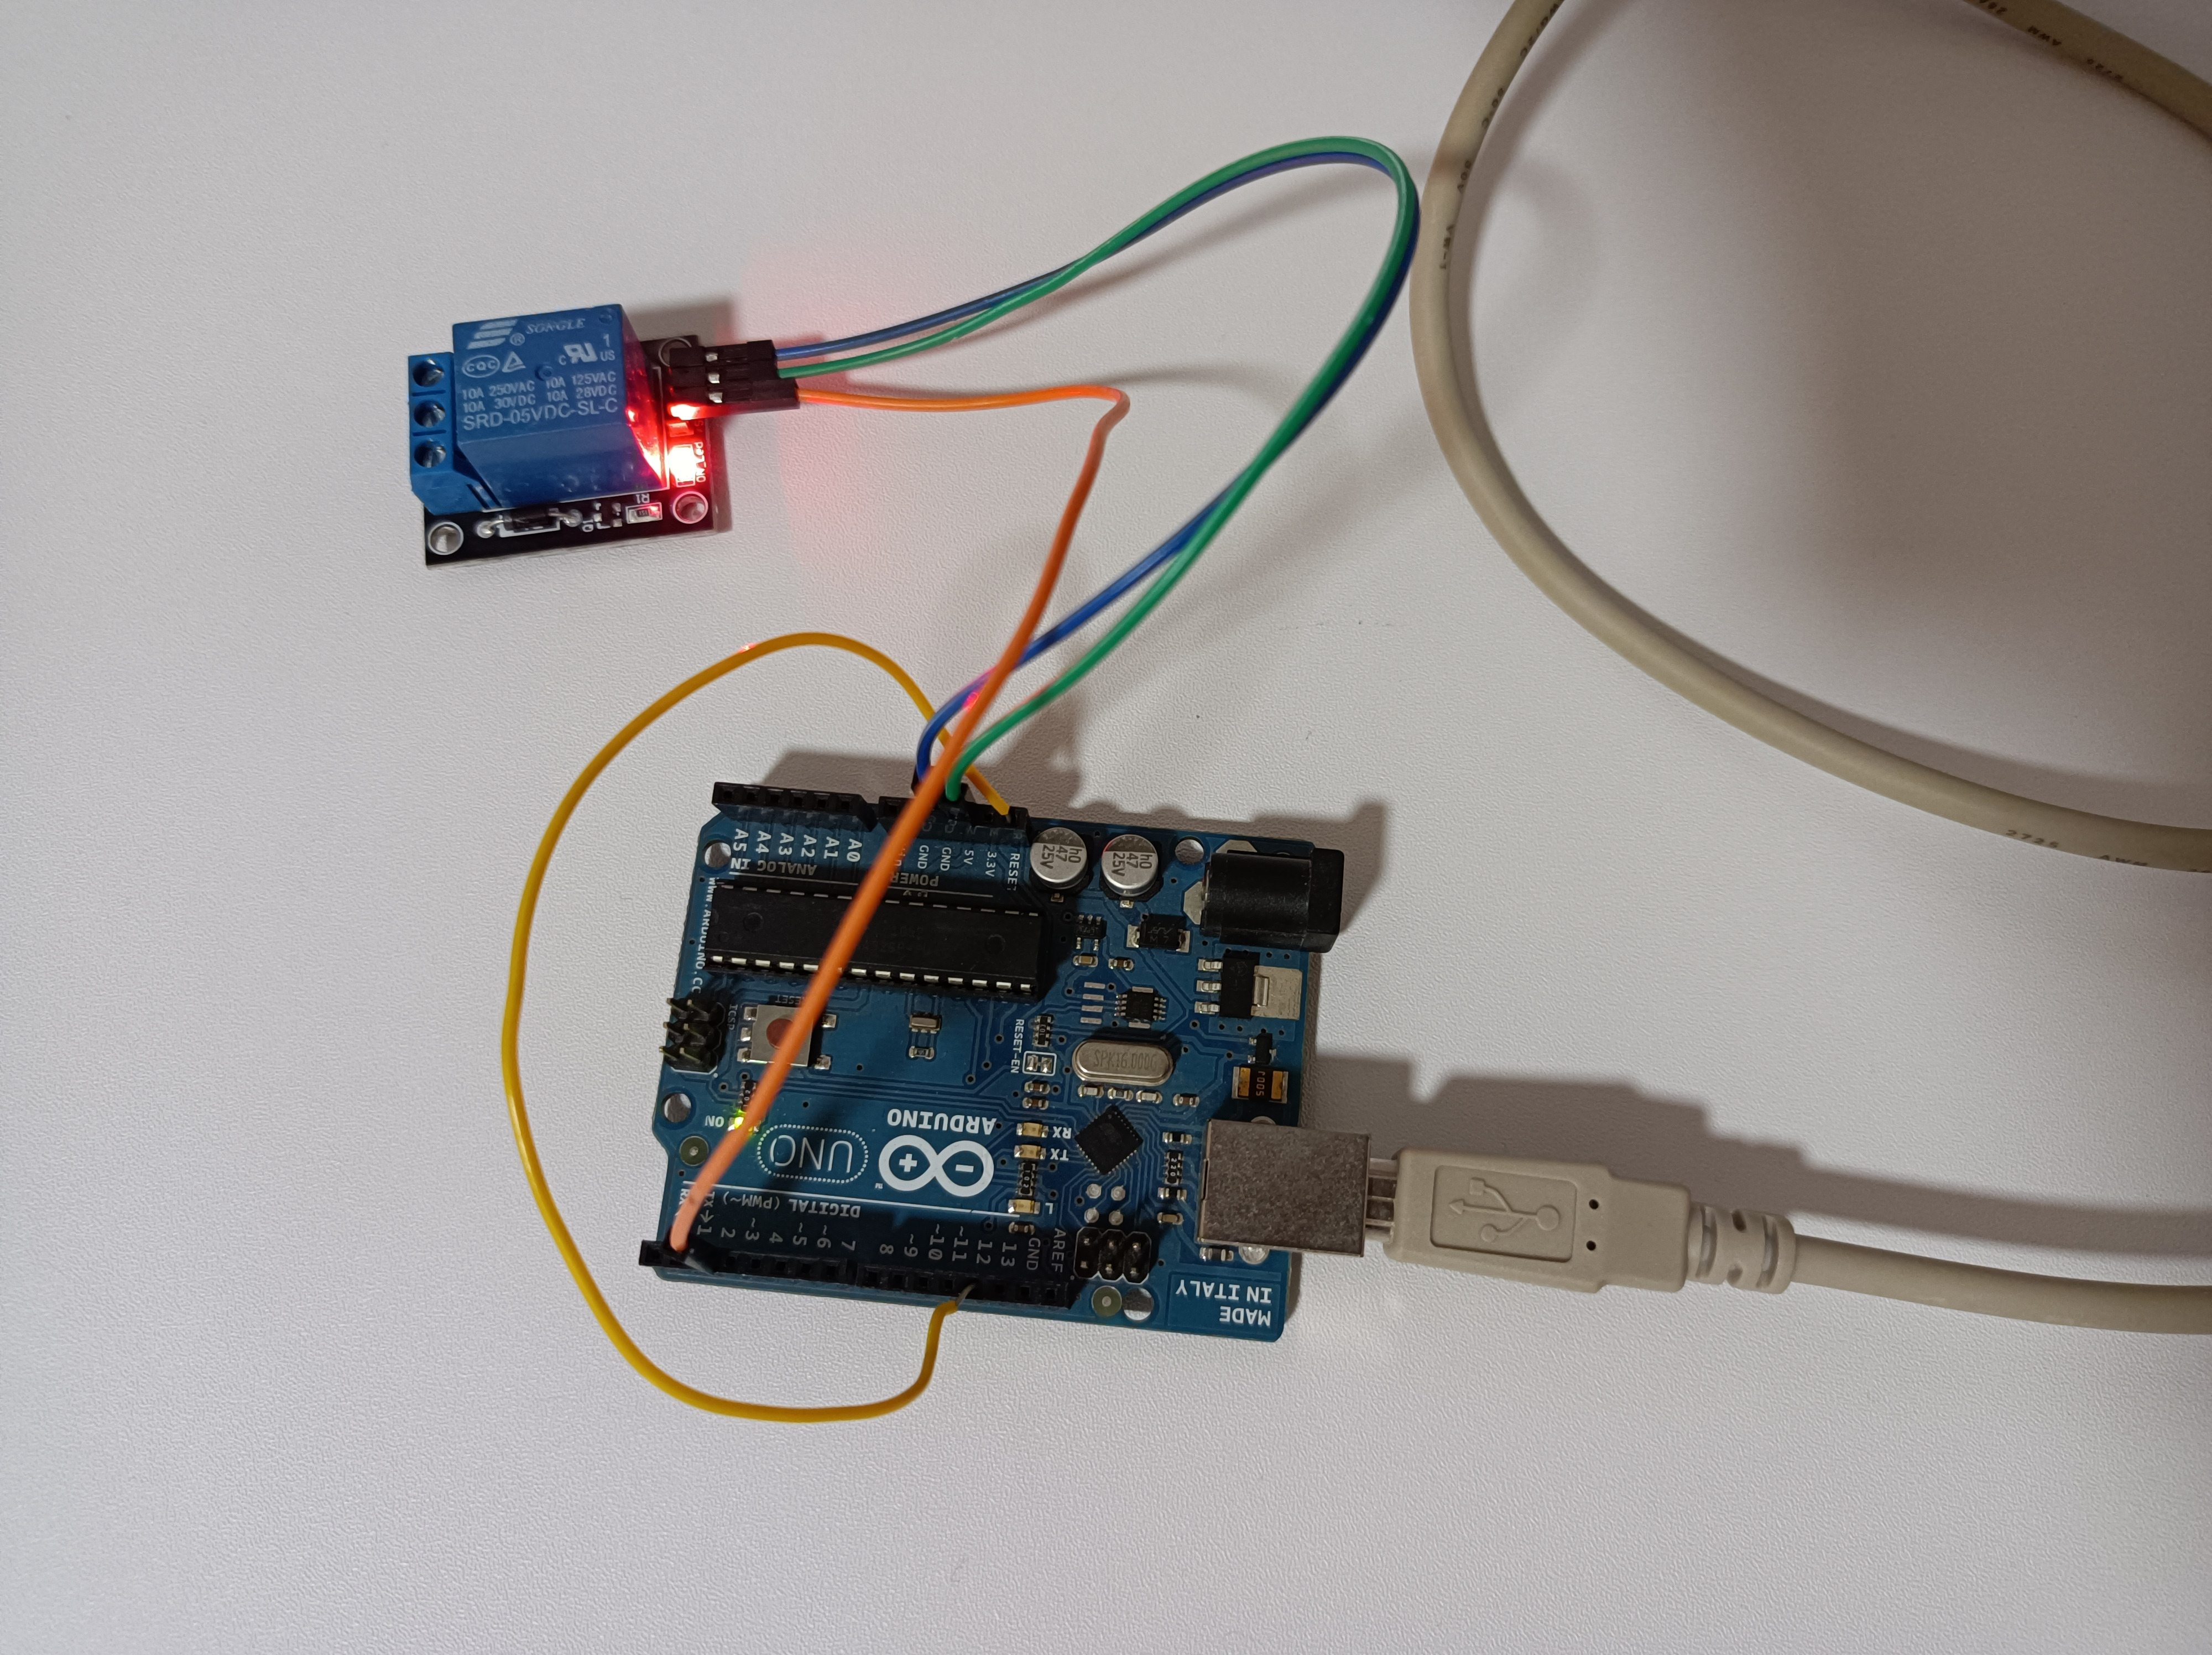
\includegraphics[width=\linewidth]{switch-light-wiring.jpg}

Programaremos la placa para que active los pines adecuados y procese las
señales que reciba por el puerto serie de manera que active el puerto serie a
9.600 bps y active el relé en caso de recibir el carácter \verb|h| y los
desactive en caso de recibir el carácter \verb|l|:

\lstinputlisting[language=C++, caption=switch-light.ino]{
    1/switch-light/switch-light.ino
}

Finalmente, desde el ordenador se enviará por el puerto serie solo las letras
\verb|h| y \verb|l| en caso de ser pulsadas, no otras, y si se pulsa \verb|q|
entonces se cerrará el programa cliente. Para ello, usaremos el lenguaje Rust
con el gestor de paquetes estándar Cargo. Estos componentes se instalan según
las indicaciones en su página
web\footnote{\url{https://www.rust-lang.org/es/tools/install}} en función del
sistema operativo que se esté usando, a través del gestor de instalaciones
Rustup. Se ha elegido este lenguaje dado que, aún estando orientado a la
programación de sistemas, garantiza que la gestión de la memoria es segura dado
que la comprueba en tiempo de compilación, esto a costa de no permitir ciertas
formas de realizar el control del flujo de ejecución.

La creación del proyecto del programa cliente se realiza ejecutando el comando
\lstinline{cargo new --vcs none nombre-del-proyecto}. En nuestro caso lo
llamaremos \verb|switch-light|, por lo que la instrucción a ejecutar será
\lstinline{cargo new --vcs none switch-light}. Esto creará una carpeta con el
nombre del mismo proyecto en el directorio desde el cual hayamos ejecutado la
instrucción, sin habilitar ningún sistema de control de versiones. Dentro de
dicha carpeta se formará una estructura de ficheros y directorios. Nos
interesan dos archivos. Por un lado está \verb|Cargo.toml|, que declara los
metadatos del proyecto y los paquetes de los que depende, con una versión
específica. Solo necesitamos añadir las dependencias después del marcador
\lstinline{[dependencies]}. Usaremos las librerías \verb|serialport|, para usar
los puertos serie del sistema, abstrayendo las diferencias entre sistemas
operativos, y \verb|console|, para acceder a características más avanzadas de
la terminal que las que proporciona la librería estándar. Este sería el
resultado:

\lstinputlisting[caption=switch-light/Cargo.toml]{
    1/switch-light/Cargo.toml
}

La versión de cada dependencia debe indicarse para evitar que cambios en la API
de las librerías impidan la compilación de la aplicación o que ésta se ejecute
de una forma inesperada.

El código del programa para realizar el comportamiento que se busca, descrito
anteriormente, es el siguiente:

\lstinputlisting[language=Rust, caption=switch-light/src/main.rs]{
    1/switch-light/src/main.rs
}

La constante \verb|PORT_PATH| debe ajustarse a la ruta del nodo de dispositivo
adecuado en Linux o al nombre del puerto donde esté conectada la placa Arduino
en el caso de Windows.

Sin embargo, hay que tener en cuenta que, como aparece comentado en el código
para la placa, en Linux hay que mantener el pin de Reset en alto, por lo que
hay que conectar dicho pin a otro que esté situado en alto, en nuestro caso el
pin 12, \emph{después de conectar la placa}, y en caso de que vaya a ser
reprogramada hay que dejar el pin de Reset libre. Esto ocurre porque Linux
envía una señal de control al abrir el puerto que Arduino interpreta como un
reset, incluso aunque se ajuste el puerto para que no envíe señales de
control\footnotemark. En Windows esto no pasa, por lo que no es necesario. El
setup mostrado ya tiene en cuenta esto, dado que se ha realizado sobre Linux.

\footnotetext{\url{https://unix.stackexchange.com/a/543527}}

Para ejecutar el programa (y compilarlo si es necesario), el comando a teclear
es \lstinline{cargo run}, dentro de la carpeta del proyecto.

En los siguientes ejercicios no se explicarán con tanto detalle las
instrucciones a ejecutar, dado que siempre siguen unos patrones muy similares.